\section{Osnovna svojstva}
\subsection{Osnovna svojstva optičkih rezonatora}
Gledamo prvo klasični odziv jednostavne Fabry-Perot (FP) rezonirajuće komore.
\begin{figure}[!h]
\begin{center}
	\includegraphics[width=9cm]{../images/F1OptMehShema.png}
\end{center}
\caption{Shema optomehaničkog sistema.}
\label{fig:F1OptMehShema}
\end{figure}

FP rezonantna šupljina sastoji se od dva visoko reflektivna
zrcala udaljena L jedno od drugog, i niz rezonancija dane s kružnom frekvencijom $\omega_{cav,m} \approx \frac{m\pi c}{L}$. Ovdje je \textit{m} cijeli broj koji označava
vibracijski mod. Razmak između dva logitudinalna rezonantna moda je dan s
\begin{equation}
	\delta\omega_{FSR} = \pi \frac{c}{L},
\end{equation}
%Nacrtaj kako izgleda neki spektar
gdje $\delta \omega_{FSR}$ označava slobodni spektralni raspon, odnosno raspon frekvencija kojim naš rezonator ne vibrira. Konačna transparentnost zrcala i
interna absorpcija ili raspršenje van rezonantne šupljine dovode do konačnog fotonske stope istjecaja $\kappa$.
Korisna je znati i optičku finesa (eng. \textit{finess}) $\mathcal{F}$ naše šupljine koja obilježava srednji broj refleksija fotona prije nego izađe iz šupljine. Dana je s
\begin{equation}
	\mathcal{F} = \frac{\delta\omega_{FSR}}{\kappa}.
\end{equation}
Optička finesa je bitna za određivanje snage unutar komore. Također možemo uvesti faktor kvalitete za optički rezonator dan pomoću
\begin{equation}
	\mathcal{Q}_{opt} = \omega_{cav} \tau.
\end{equation}
\begin{Bilješka}
Recimo da je snaga lasera za pumpanje komore prije ulaska u komoru 1W. Recimo da je reflektivnost visoko reflektivnih zrcala 0,99999.
U komoru će ući $\left(1-1\cdot0,99999\right)$ W snage zračenja. Ako je $\mathcal{F}=100000$ snaga zračenenja u komori će biti
$\left(1-1\cdot0,99999\right)\cdot 100000 = 1W$ prije nego iscjedi zračenje iz komore u vremenu $\kappa^{-1} = \tau$, što je u ovom primjeru isto kao i snaga ulaznog zračenja.
\end{Bilješka}
Općenito stopa istjecanja $\kappa$ može imati dva doprinosa: Od korisnog ulaznog (izlaznog) vezanja, $\kappa_{ex}$ i od unutarnjih gubitaka, $\kappa_0$. Tako da možemo pisati
\begin{equation}
	\kappa = \kappa_{ex} + \kappa_0.
\end{equation}

